\documentclass[twocolumn]{aastex62}

\usepackage[utf8]{inputenc}
\usepackage{xspace}
\usepackage{url}
\usepackage{listings}
\usepackage{inconsolata} % standard "prettier" astropy latex font

\newcommand{\package}[1]{\texttt{#1}\xspace}
\newcommand{\astroquery}{\package{astroquery}}
\newcommand{\astropy}{Astropy\xspace}
\newcommand{\astropypkg}{\package{astropy}}

\definecolor{dkgreen}{rgb}{0,0.6,0}
\definecolor{gray}{rgb}{0.5,0.5,0.5}
\definecolor{mauve}{rgb}{0.58,0,0.82}

\renewcommand{\lstlistingname}{Example}
\lstset{frame=tb,
  language=Python,
  aboveskip=3mm,
  belowskip=3mm,
  showstringspaces=false,
  columns=flexible,
  basicstyle={\small\ttfamily},
  numbers=none,
  numberstyle=\tiny\color{gray},
  keywordstyle=\color{blue},
  commentstyle=\color{dkgreen},
  stringstyle=\color{mauve},
  breaklines=true,
  breakatwhitespace=true,
  tabsize=3,
}

\begin{document}
\newcommand{\nraojansky}{\affiliation{\it{Jansky fellow of the National Radio Astronomy Observatory, 1003 Lopezville Rd, Socorro, NM 87801 USA }}}

\author[0000-0001-6431-9633]{Adam Ginsburg}
\nraojansky

\correspondingauthor{Adam Ginsburg}
\email{aginsbur@nrao.edu; adam.g.ginsburg@gmail.com}

\author{Brigitta Sipocz}

\author[0000-0003-2528-3409]{Brett M. Morris}
\affiliation{Astronomy Department, University of Washington, Seattle, WA 98195, USA}

\author[0000-0002-8642-1329]{Thomas P. Robitaille}
\affiliation{Aperio Software Ltd., Headingley Enterprise and Arts Centre, Bennett Road, Leeds, LS6 3HN, United Kingdom}

\author[0000-0001-9898-5597]{Leo P. Singer}
\affiliation{Astroparticle Physics Laboratory, NASA Goddard Space Flight Center, Mail Code 661, Greenbelt, MD 20771, USA}
\affiliation{Joint Space-Science Institute, University of Maryland, College Park, MD 20742, USA}

\author{the Astroquery collaboration, a subset of the astropy collaboration}


\title{\astroquery: An Astronomical Web-Querying Package in Python}

\begin{abstract}
\astroquery is a collection of tools for requesting data from databases hosted
on remote servers with interfaces exposed on the internet, including those with
web pages but without formal application program interfaces (APIs).  These
tools are built on the Python
\package{requests} package, which is used to make HTTP requests, and
\astropypkg, which provides most of the data parsing functionality. \astroquery
has received significant contributions from throughout the astronomical community,
including several significant contributions from telescope archives.
\astroquery enables the creation of fully reproducible workflows from data
acquisition through publication.  This document describes the philosophy, basic
structure, and development model of the \astroquery package.
The complete documentation for astroquery can be found at
\url{http://astroquery.readthedocs.io/}.
\footnote{%
The repository associated with this paper is:\\
\url{https://github.com/adamginsburg/astroquery-paper}
}
\end{abstract}


\section{Introduction}
%Sharing data is a critical component of astronomical research.  Astronomy
%has historically been a leading field in data sharing, motivated at least
%in part by questions that cannot be answered with single instruments.
In the past few decades, large-scale surveys have played a huge role in
advancing our understanding of the universe, and these surveys have produced
enormous reservoirs of data that astronomers regularly access.  However, tools
for accessing these reservoirs are heterogeneous and often only available via
graphical user interfaces (GUIs) such as web sites.

One of the cornerstones of research is reproducibility. To be able to reproduce
research, the data need to be available to everyone. Many scientific journals
encourage or demand that the underlying data  accompany the article or be
uploaded to a hosting service. Data sharing is not only important for new
results, but also to provide the ability to test and verify published results.
While many different efforts to promote data sharing have made the practice
more common, it is difficult to keep track of how and where to retrieve a given
data set. A common scripted interface to tie all these services together is a
good way to make all the different data more accessible, and it provides
authors with the ability to make the full analysis process they used -- from
data download to publication -- repeatable.  A centrally maintained library
also safeguards against inevitable `link rot' on data archives, moving some of
the responsibility for maintaining long-term reproducibility from the
individual researcher to the broader community.

Data sharing has taken on a variety of forms.  The most prominent are the
major observatory archives: MAST, NOAO, ESO, ESA, IPAC, CDS, NRAO, CXC, HEASARC,
and CADC are the main organizations hosting raw and processed data from
ground and space based telescopes.  These data archives also serve as the
primary means for serving data to users when the data are taken in queue
mode, i.e., when the data are taken while the observer is not on-site.

In addition to observatories and telescopes, individual surveys often share
their full data sets.  In some cases, these data sets are shared via the
observatory that acquired them, for example, the all-sky data acquired with
Planck, WMAP, and COBE\@.  Other surveys, particularly ground-based surveys,
serve their own data.  Examples include SDSS, 2MASS, UKIDSS, and VSA.

%TODO: mention data collector sites, too, nasa\_exoplanet\_archive, simbad,
%skyview, OAC, etc.

Individual teams and small groups often share their data via their own
custom websites.  These services do not follow any particular standard and can
be widely varied in the type and amount of data shared.  Sometimes these data
are shared via the archive systems (e.g., IRSA at IPAC hosts many individual
survey data sets), while others use their own web hosting systems \citep[e.g.,
MAGPIS;][]{Helfand2006}.

Finally, there are other data types relevant to astronomy that are not
served by the typical astronomical databases.  Examples include databases of
molecular and atomic properties, such as those provided by Splatalogue and
the NIST Atomic Spectra Database, or services that are computationally
intensive or require constant updates, like Solar System ephemerides
provided by services like JPL HORIZONS, or the Minor Planet Center.

\astroquery arose from a desire to access these databases from the Python command line
in a scriptable fashion.  Script-based data access provides astronomers with
the ability to make reproducible analysis scripts and pipelines in which the data are
acquired and processed into scientifically relevant results with minimal
user interaction.

In this paper, we provide an overview of the \astroquery package.  Section
\ref{sec:software} describes the basic layout of the software and the shared
API concept underlying all modules.  Section \ref{sec:development} describes
the development model.  Finally, Section \ref{sec:documentation} describes how
\astroquery is documented.

% The Virtual Observatory has some overlap with astroquery, but it does not
% provide the simple tools many astronomers find necessary in day-to-day work.
% Additionally, many of the services noted above do not support VO standards or
% protocols and are therefore inaccessible to the VO.


\section{The Software}
\label{sec:software}
\astroquery consists of a collection of modules that mostly share a similar
interface, but are meant to be used independently.  They are primarily based on
a common framework that uses the Python \package{requests} package to perform
HTTP requests to communicate with web services.

For new service development, there is a \texttt{template\_module} that lays
out the basic framework of any new module.  All modules have a single core
\texttt{class} that has some number of associated \texttt{query\_*} methods.
The most common query methods are \texttt{query\_region}, which usually
provide a ``cone search'' functionality, i.e., they search for data within a
circularly symmetric region projected on the sky. The returned results of
the queries then are returned in an \astropypkg
\citep{Astropy-Collaboration2018, Astropy-Collaboration2013}
\texttt{Table}\footnote{\url{http://docs.astropy.org/en/stable/table/}}.

An example using the SIMBAD interface is shown below:\footnote{see
\url{http://astroquery.readthedocs.io/en/latest/simbad/simbad.html}}
\begin{lstlisting}[caption=Query SIMBAD for a region around M81]
from astroquery.simbad import Simbad
result_table = Simbad.query_region("m81")
\end{lstlisting}
In this example, \texttt{Simbad} is an instance of the
\texttt{astroquery.simbad.SimbadClass} class.

While there is a common suggested API described in the \texttt{template\_module},
individual packages are not \emph{required} to support this API because, for
some, it is not possible.  For example, the atomic and molecular databases refer
to physical data that is not related to positions on the sky and therefore
their \astroquery modules cannot include \texttt{query\_region} methods. The
same applies to Solar System object ephemerides queries. Differences in the API
are discussed in the \astroquery documentation (see Section
\ref{sec:documentation}).

\subsection{Version Numbers}
\label{sec:versionnumbers}
\astroquery uses the same format as traditional semantic versioning,
with versions indicated in the format \texttt{MAJOR.MINOR.PATCH.devCOMMIT\_ID} (for
example, \texttt{0.3.9.dev4581}).

\astroquery patches are frequently made to accommodate upstream changes, i.e.,
changes made to the remote service, and as such are not guaranteed to be
backward-compatible. Thus, starting in mid-2018, \astroquery switched from a manual release model to a
continuous deployment model.  Prior to this change, the
\texttt{MAJOR.MINOR.PATCH} versions were each created manually by one of the
maintainers, then pushed to package release services.  After this change, each
accepted pull request automatically triggered a new release via the python
package index\footnote{\url{https://pypi.org/}}.


%\subsection{Versioning}
%Unlike the core \astropypkg package, \astroquery exists in an `always-unstable' state.
%Because \astroquery relies on remote services' APIs to function, changes to those
%APIs may break \astroquery without warning.  We have
%frequent releases to accommodate remote changes.  Starting in 2018, \astroquery
%moved to a `continuous release' model, in which every change merged into the
%master branch is deployed as a release on the python package index (pypi).
%
%Some services have been helpful about alerting the \astroquery development team
%in advance when API changes are imminent.  We are grateful for such advance
%warning and encourage other services to check in and file issues on \astroquery's
%issue tracker when significant API modifications are made.

\subsection{HTTP User-Agent}
\label{sec:useragent}
\astroquery identifies itself to host services using the \texttt{HTTP
User-Agent} header data.  The format of the User-Agent string is:
\[\texttt{astroquery/\{version\} \{requests\_version\}}\] where
\texttt{\{version\}} is a version number of the form described in \S
\ref{sec:versionnumbers} and \texttt{\{requests\_version\}} is the
corresponding version of the Python \package{requests} package. For example:
\[\texttt{astroquery/0.3.9.dev4863 python-requests/2.14.2}\]
This information
can be used by data hosting services to determine how many users are accessing
their service via \astroquery and to assist in debugging if improper queries
are being submitted.


\subsection{The API}
The common API has a few features defined in the \texttt{template\_module}.
Each service is expected to provide the following interfaces, assuming they are
applicable:

\begin{itemize}
    \item \texttt{query\_region} - A function that accepts an \astropypkg
        \texttt{SkyCoord} object representing a point on the sky plus a
        specification of the radius around which to search.
        The returned object is an \astropypkg \texttt{Table}.
    \item \texttt{query\_object} - A function that accepts the name of an
        object.  This method relies on the service to resolve the object name, i.e., it does not use a name resolver
        like \texttt{SESAME}\footnote{\url{http://cds.u-strasbg.fr/cgi-bin/Sesame}}.
        The returned object is an \astropypkg \texttt{Table}.
    \item \texttt{get\_images} - For services that provide image data, this
        function accepts an \astropypkg \texttt{SkyCoord} and a radius to search for data
        that cover the specified target. The returned object is a list
        of \texttt{astropy.io.fits.HDUList} objects.

\end{itemize}

Beyond these basic methods, there is a series of functions with the same
names, but with the additional suffix \texttt{\_async}.  The
\texttt{query\_*\_async} functions return a \texttt{requests.Response} object
from the accessed website, providing developers with
the ability to access the data in a stream or access only the response
metadata (i.e., the \texttt{async} methods do not download the corresponding
data, so they may be useful for collecting metadata for very large files).  The
\texttt{get\_images\_async} method returns
\texttt{FileContainer} objects that similarly provide `lazy' access to the
data, but specifically for FITS files.  Contributors need only implement
these \texttt{\_async} functions because a wrapper tool exists to convert
\texttt{\_async} functions into their corresponding non-asynchronous versions.

Deviations from this standard API are documented in the \astroquery
documentation (see Section \ref{sec:documentation}).

\subsection{Caching and login functionality}
For new module development, there are tools provide to handle various aspects
of querying that are common across all modules.  The \texttt{BaseQuery}
metaclass provides tools for caching requests and downloaded data, reducing the
network load for repeated queries.  Cached data are stored in the user's
\texttt{~/.astropy/cache/astroquery} directory.  The \texttt{BaseQuery}
metaclass is also responsible for setting the User-Agent (\S
\ref{sec:useragent}).  The \texttt{QueryWithLogin} metaclass provides a
framework for secure logging in to services that require user
authentication.



\subsection{Testing}
\astroquery testing is somewhat different from most other packages in the Python
ecosystem.  While the tests are based on the \astropypkg testing infrastructure and use
\package{pytest} to run and check the outputs, the \astroquery tests are split into
\emph{remote} and \emph{local}.  The remote tests exactly replicate what a user
would enter at the command line, but they are dependent on the stability of the
remote services.

In our experience it is quite rare for all of the \astroquery-supported
services to be accessible simultaneously. We therefore require that each
module provide some tests that do not rely on having an internet connection.
These tests rely on \emph{monkeypatching}\footnote{Monkeypatching is the
  dynamic replacement of attributes at runtime, i.e., changing what
  functions do after they are imported.} to replace the remote
requests. Instead of downloading data, the test suite uses locally available
files to test the query mechanisms and the data parsers.  Monkeypatching in
the context of \package{pytest} results in code that is generally more
difficult to understand than typical Python code, but a set of tests
independent of the remote services is necessary.

The local tests are run as part of the continuous integration for the
project with each commit.  The remote tests are run for merges and as part of a
regularly-scheduled \texttt{cron} job.  Running the remote tests less frequently
helps reduce the burden on the remote services.

\subsection{Other utilities}
There are several general-use utilities implemented as part of \astroquery, such
as a bulk FITS file downloader and renamer and a download progressbar.  There
is also a schema system implemented to allow user-side parameter validation.
The schema tool is only implemented in the ESO and Vizier modules, but it could
be expanded to other modules to reduce the number of doomed-to-fail queries
sent through \astroquery.

\section{Development history and status}
\label{sec:development}
Anyone can contribute to \astroquery.  The maintainers are committed to helping
developers make new modules that meet the requirements of \astroquery.  This
section describes how \astroquery has been developed, but we welcome all sorts
of new contributions, including new modules, upgrades to existing modules, and
minor corrections to existing tools.

\astroquery is an \astropy coordinated package \citep{APE15} and is a critical
component of the \astropy Project ecosystem \citep{Astropy-Collaboration2018}.
It is a standalone project and will remain independent of the \astropypkg core
package\footnote{Many \astropy affiliated packages are developed with the
intent of eventually including them in the core of \astropypkg.  In contrast,
\astroquery intends to remain a separate package indefinitely largely because
of its need to rapidly adapt to changes in the remote services; \astropypkg
cannot make such rapid changes because users rely on its stability.}, but is
coordinated by the \astropy Project to ensure sustainability and maintenance.

\astroquery has received contributions from 77 people as of August 2018.  While the primary maintenance
burden is shouldered by two people at any given time (the first two authors),
most individual modules have been implemented independently by interested
contributors.

Some contributions have come with direct institutional support.  The ESA Gaia and
ESASky modules were provided and supported by developers working for ESA\@.  The
MAST and VO Cone Search query tools were added by developers at STScI, with the
latter moved over from \texttt{astropy.vo} (see Section \ref{sec:vo}).

\astroquery also receives contributions from other funded programs. For instance, the
JPLHorizons module has been implemented as part of the \texttt{sbpy}
project\footnote{\url{http://sbpy.org}} with support from NASA PDART grant
80NSSC18K0987. Further Solar System-related services are planned to be added to
\astroquery through this support.

\astroquery has received support from the Google Summer of Code
program, with two students (co-authors Madhura Parikh and Simon Liedtke)
from 2013--2014.



\subsection{Relation to the VO}
\label{sec:vo}

The Virtual Observatory (VO) has some goals similar to \astroquery,
though their approach and philosophy is different.  Where VO services provide a
single point of access for all VO-compatible services, \astroquery
provides a collection of access points that do not require a specific API from
the hosting service.  The general philosophy in \astroquery is to
replicate the web page interface provided by a given service as closely as
possible.  While this approach makes some versions of cross-archive searches
more difficult, it keeps the barrier to entry for new users fairly low and limits
the maintenance burden for upstream developers.

However, there are developments in progress to allow more VO-like queries
within \astroquery, such as searching for databases by keywords.  As more
services implement VO-based access, some query modules may adopt VO as a backend,
but these changes should be transparent to users (i.e., the \astroquery
interfaces will remain unchanged).  The documentation may guide users on how
to use the more sophisticated VO tools that underly these tools


Some general VO tools are available in astroquery.  The \texttt{vo\_conesearch}
package, which originally resided in \astropypkg, is now part of \astroquery.  VO
Cone Search has a \texttt{query\_region} interface like the other \astroquery
services in addition to the existing interfaces ported over from \astropypkg.
As of \astropypkg 3.0, \texttt{astropy.vo} no longer exists; therefore,
\astroquery is now the primary provider of this VO Cone Search service. From a
typical user's standpoint, switching over from \texttt{astropy.vo} should
result in no difference except for updating their Python \texttt{import}
statements (e.g., \texttt{from astroquery.vo\_conesearch import conesearch}
instead of \texttt{from astropy.vo.client import conesearch}).



\section{Documentation and References}
\label{sec:documentation}
\subsection{Online documentation}
The \astroquery modules are documented online and can be accessed through
readthedocs at \url{https://astroquery.readthedocs.io/en/latest/}.
We include one detailed example of how to use \astroquery in Appendix \ref{sec:example},
but interested users will find many more on the documentation page and
in the example gallery (\url{https://astroquery.readthedocs.io/en/latest/gallery.html}).

\section{Summary}
\astroquery is a toolkit for accessing remotely hosted data through Python.
It is part of the \astropypkg affiliated package system.
We have described its general layout and development model.
We welcome any new contributions.


\bibliographystyle{aasjournal}
\bibliography{bibliography}

\appendix
\section{Example}
\label{sec:example}
In this appendix, we show an example of \astroquery in action, highlighting the
ability to use multiple modules and interact with \astropypkg's table, coordinate,
and unit tools.  This example approximately reproduces Figure 1 of
\citet{Eisner2016a}, but with a different background.  It can also be found on
\astroquery's gallery page
(\url{http://astroquery.readthedocs.io/en/latest/gallery.html}).
Another illustration of how to use astroquery tools in a finder chart making
tool is \texttt{fcmaker}, which produces charts for ESO observations using
\astroquery \citep{Vogt2018a}.


\newpage
\lstinputlisting[frame=single]{example1.py}


\begin{figure*}[!htp]
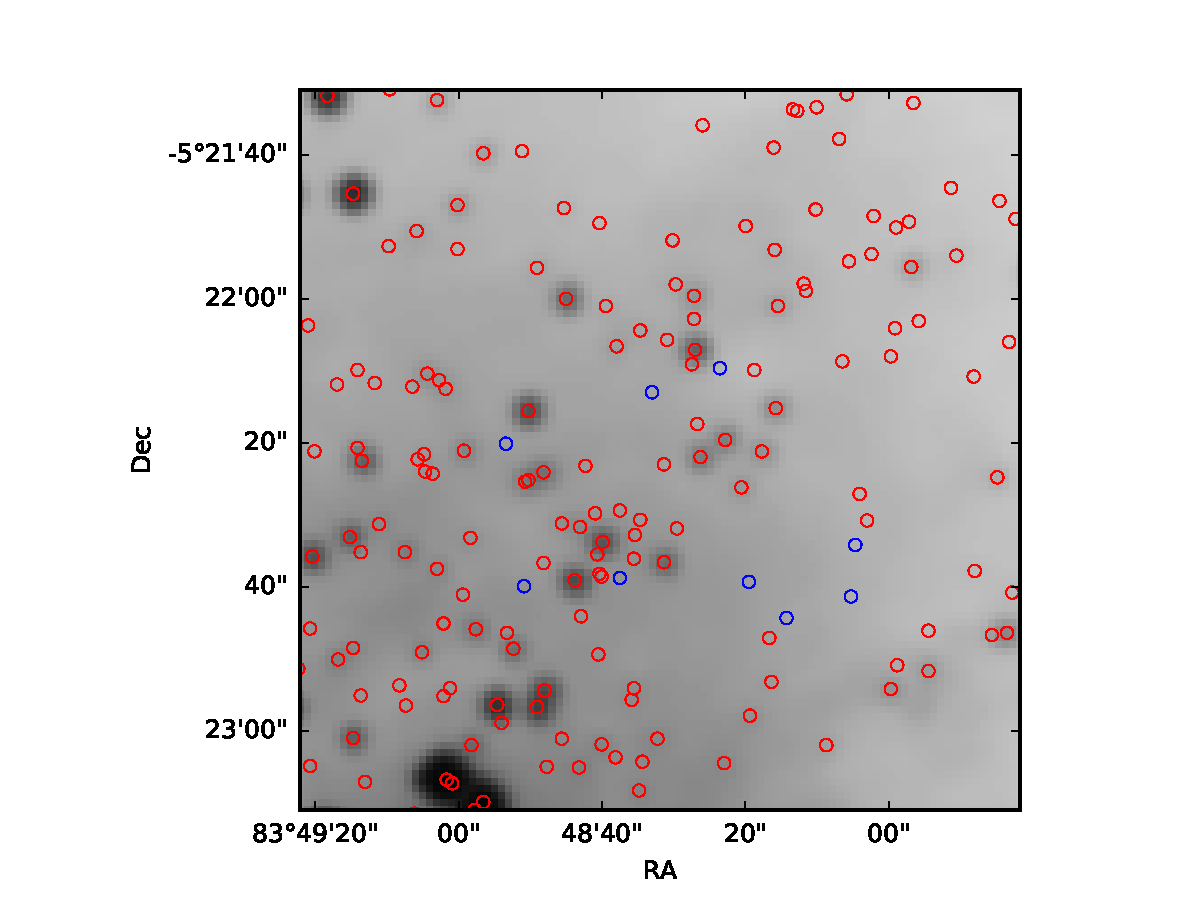
\includegraphics[scale=1,width=7in]{example_figure_1.pdf}
\caption{An example figure made using \astroquery's \texttt{skyview} and
\texttt{vizier} modules with \astropypkg's \texttt{table}, \texttt{coordinates},
\texttt{units}, and \texttt{wcs} modules.  The blue stars show sources from
an older, less complete catalog and the red circles show sources from a more
recent, more complete catalog.
}
\label{fig:example1}
\end{figure*}

\end{document}
